\section{Extended MCA: Showing interactions in $2^Q$ tables}\label{sec:ca-mcainter}
\ixon{multiple correspondence analysis!extended}
As we discussed earlier,
MCA was developed as a way to depict the relationships among the
categories of multiple categorical variables, and the derivation of
the method based on the Burt matrix implies that only the relations
in the bivariate marginal tables are represented in the displays.
\ix{Burt matrix}
This is based on the assumption \citep{Gifi:90,Greenacre:88}
that, as with multivariate normal data, the structural relations
among variables are adequately captured by bivariate associations.%
\footnote{Another concern is that higher-way \ctab s may become
sparse, hence resulting in instability in solutions
\citep{Heijden:87}.}
These developments, and usually practice, have led to the mistaken beliefs that,
\begin{seriate}
\item MCA can \emph{only}
represent bivariate (first-order) interactions,
\item MCA can \emph{only} portray the category points of the variables
(not their combinations), and
\item associations must be inferred from the relative positions of
the category points.
\end{seriate}

A recent paper by \citet{MeulmanHeiser:97} demonstrates, however,
that none of these are necessary consequences of MCA itself.
Moreover, for the case of binary variables (a $2^Q$ table),
an odds interpretation of distances between category points
leads to simple geometrical patterns in MCA plots.

Their method for including higher-order effects involves adding all cross-terms,
up to a given order,
to the set of variables in frequency form which are analyzed by
MCA.  For example, with three variables, $A$, $B$, and $C$,
generate all interaction terms (using the \texttt{|} syntax of
\PROC{GLM} or \PROC{CATMOD}),
\begin{equation*}
\mbox{\texttt{A | B | C}} \iff \mbox{\texttt{A B C A*B A*C B*C A*B*C}}
\end{equation*}
\begin{table}[htb]
 \caption[Extended factor matrix for a $2\times 2\times2$ table]%
         {Extended factor matrix for a $2\times 2\times2$ table, including all possible cross-classifications.}\label{tab:mcadesign}\vspace{5pt}
\begin{center}
\begin{tabular}{lll | ccc ccc c}
 \hline
       &       &        &  A  &  B  &  C  &  AB &  AC &  BC & ABC \\ \hline
 $a_1$ & $b_1$ & $c_1$  &  1  &  1  &  1  &  1  &  1  &  1  &  1 \\
       &       & $c_2$  &  1  &  1  &  2  &  1  &  2  &  2  &  2 \\
       & $b_2$ & $c_1$  &  1  &  2  &  1  &  2  &  1  &  3  &  3 \\
       &       & $c_2$  &  1  &  2  &  2  &  2  &  2  &  4  &  4 \\
%
 $a_2$ & $b_1$ & $c_1$  &  2  &  1  &  1  &  3  &  3  &  1  &  5 \\
       &       & $c_2$  &  2  &  1  &  2  &  3  &  4  &  2  &  6 \\
       & $b_2$ & $c_1$  &  2  &  2  &  1  &  4  &  3  &  3  &  7 \\
       &       & $c_2$  &  2  &  2  &  2  &  4  &  4  &  4  &  8 \\
%
\end{tabular}
\end{center}
\end{table}

Similarly, the \texttt{@} syntax specifies all terms up to a given
order; for example,
\begin{equation*}
\mbox{\texttt{A | B | C | D}@2} \iff \mbox{\texttt{A B C D A*B A*C A*D B*C B*D C*D}}
\end{equation*}
generates all
terms up to order 2.  To illustrate, \tabref{tab:mcadesign} shows all terms
for the three-way model \texttt{(A | B | C)}.
Like any \pname{CLASS} variables, it is only necessary for the variable
values to be discrete.
However, it is strictly necessary to include \emph{all} terms at the same
interaction level, up to the given order.

The indicator matrix will then consist of the dummy variables for
these terms, so that, for \tabref{tab:mcadesign},
$\mat{Z} = [
 \mat{Z}_A  \mat{Z}_B  \mat{Z}_C  \mat{Z}_{AB}
 \mat{Z}_{AC}  \mat{Z}_{BC}  \mat{Z}_{ABC}
]$.
Forming the Burt matrix, $ \mat{B} =  \mat{Z}\trans  \mat{Z}$,
we see that the off-diagonal blocks now contain \emph{all}
contingency tables which can be formed from the original variables
(up to the specified order), not just the pairwise bivariate
tables.
The category points for an MCA solution based on this
extended $\mat{Z}$ matrix will then contain, in addition to the
usual one-way ``main effect'' points
of the variables themselves, sets of interaction points
(e.g., $(ab)_{ij}$, $(ac)_{ik}$, and so forth) for the various
combinations of factors included.

What happens to the category points for these interaction terms in the MCA
solution?
\citet{MeulmanHeiser:97} demonstrate the remarkable results that
\begin{itemize*}
\item distance ratios between sets of interaction points correspond to
odds ratios in the higher-order table,
and
\item the various independence structures we have considered
(cf. \tabref{tab:hyp3way})
give rise to simple configurations of points in the category
space.
\end{itemize*}

For simplicity, consider a $2\times 2$ table with cell probabilities
$p_{ij}$.  Let $\vec{z}_{ij}$
refer to the profile coordinate points for the $(ab)_{ij}$
combinations, and let $\vec{z}_{i\bullet}$, $\vec{z}_{\bullet j}$
be the coordinate points for the one-way $A$ and $B$ effects,
respectively.  Then, the  $\vec{z}_{ij}$ define a quadrilateral,
and the $\vec{z}_{i\bullet}$ and $\vec{z}_{\bullet j}$ are the
centroids (weighted by $p_{ij}$) of the corresponding corners,
as shown in \figref{fig:mcaidemo}.  In this figure, the mass, $p_{ij}$ of each cell point is indicated by its size and the $z$ points are labeled
by their subscripts.

\begin{figure}[htb]
  \centering
  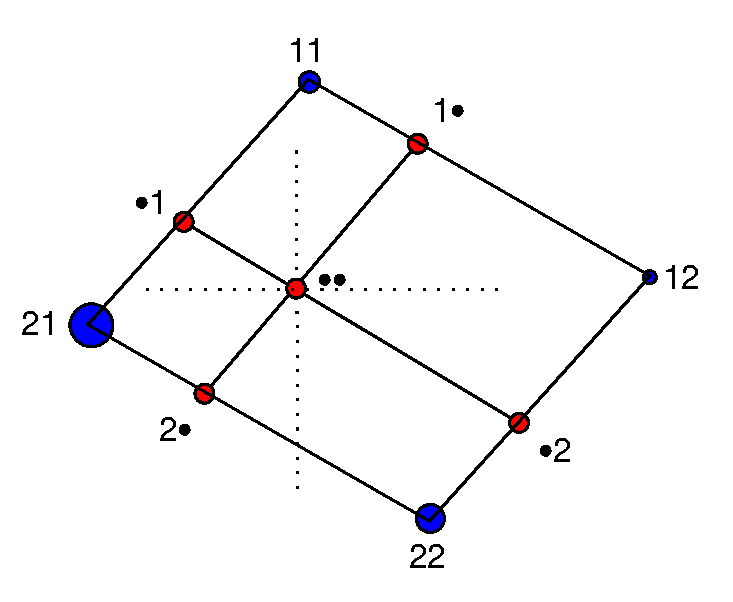
\includegraphics[scale=.9,clip]{ch5/fig/mcaidemo}
  \caption[Category points and profile points in extended MCA representation]{Category points ($\vec{z}_{ij}$) and profile points
  ($\vec{z}_{i\bullet}$, $\vec{z}_{\bullet j}$) in extended MCA representation. Under independence, the lines connecting the profile points are parallel to those connecting corresponding category points.}\label{fig:mcaidemo}
\end{figure}
The centroid points are related to the interaction points as (weighted)
linear combinations:
\begin{eqnarray*}%\label{eq:mcainter1}
  \vec{z}_{i \bullet} & = &
   \frac{p_{i1}}{p_{i+}} \: \vec{z}_{i1} +
   \frac{p_{i2}}{p_{i+}} \: \vec{z}_{i2} \\
  \vec{z}_{\bullet j} & = &
   \frac{p_{1j}}{p_{+j}} \: \vec{z}_{1j} +
   \frac{p_{2j}}{p_{+j}} \: \vec{z}_{2j}
\end{eqnarray*}
Now, for any edge of the quadrilateral, e.g., $z_{i1}$, $z_{i2}$,
their centroid is located on the line between them, so the
distances must be additive,
\begin{equation*}%\label{eq:mcainter2}
  d( \vec{z}_{i1}, \vec{z}_{i2} ) =
  d( \vec{z}_{i1}, \vec{z}_{i \bullet} ) +
  d( \vec{z}_{i \bullet}, \vec{z}_{i2} )
\end{equation*}
From these relations, \citet{MeulmanHeiser:97} show that:
\begin{itemize}
\item Given $A=i$ (or, $B=j$), the odds of being in category 1 vs. category 2
of $B$ (or $A$) are shown in the display by the inverse ratio of their
distances to their centroid.  For example,
\begin{equation*}%\label{eq:mcainter3}
  \frac{p_{i1}}{p_{i2}} =
  \frac{ d( \vec{z}_{i2}, \vec{z}_{i \bullet} ) }
       { d( \vec{z}_{i1}, \vec{z}_{i \bullet} ) }
\end{equation*}
\item The odds ratio $\theta$ has a simple multiplicative relation
to these distances among the four corner points and their
centroids.
\begin{equation}\label{eq:mcainter4}
  \theta =
  \frac{p_{11} p_{22}}{p_{12} p_{21}} =
  \frac{ d( \vec{z}_{12}, \vec{z}_{\bullet 2}) \: d( \vec{z}_{21}, \vec{z}_{\bullet 1} )}
       { d( \vec{z}_{11}, \vec{z}_{\bullet 1}) \: d( \vec{z}_{22}, \vec{z}_{\bullet 2} )}
\end{equation}
\item Under independence, $\theta =1$, and \eqref{eq:mcainter4}
therefore implies that
(a) the corner points form a parallelogram, and
(b) the lines connecting the centroids of the same variable
(e.g., $(\vec{z}_{\bullet 1}, \vec{z}_{\bullet 2}))$ are parallel
to those of their respective category points.
These relations of parallelism and additivity are shown in \figref{fig:mcaidemo}.
\end{itemize}

Although this discussion was presented
in terms of a $2 \times 2$ table, the geometrical relations extend
directly to \emph{any} number of binary variables.
For a $2 \times 2 \times 2$ table,  the models of various types of
independence shown in \tabref{tab:hyp3way} can all be characterized
in terms of the three odds ratios for all pairs of variables, and
therefore in terms of parallelism and additivity of the corresponding
pairwise quadrilaterals in the spatial representation.
Essentially, each independence relation corresponds to one odds ratio $\theta=1$,
which in turn is shown as one two-way term whose profile points form
a parallelogram, as shown in the table below.
 \begin{center}
 \begin{tabular}{lll c}
 \hline
            &  Independence  &             &  Number of parallel    \\
Hypothesis  &  relations     & Odds ratios &  two-way profile sets  \\ \hline
$H_1$  & $A \perp B \perp C$ &  $\theta_{AB} = \theta_{AC} = \theta_{BC} = 1$ & 3 \\
%
$H_2$  & $A , B \perp C$     &  $\theta_{AC} = \theta_{BC} = 1$ & 2 \\
%
$H_3$  & $A \perp B \given C$ &  $\theta_{AB} = 1$               & 1 \\
%
$H_4$  & none                & all $\theta \neq 1$               & 0 \\
%
  \hline
 \end{tabular}
 \end{center}


The following example demonstrates these ideas with a $2^3$ table, where
one two-way term is independent by design.
It also illustrates how to generate the interaction
variables, and some special techniques for displaying the extended
MCA solution.

\begin{Example}[bartlett]{Bartlett's data}
In a classic paper that extended the notion of interaction to three-way
tables, \citet{Bartlett:35} gave the data shown in \tabref{tab:bartlett}
from an experiment designed to investigate the propagation of
plum root stocks from cuttings.
In the $2 \times 2 \times 2$ table, time of planting (T) and length
of cutting (L) are factors; whether the cutting was alive or dead (A)
was the response.
Note that the column totals for the factors are all equal,
these having been fixed by the experimental design.
Thus, there can be
no $T\times L$ marginal association, and interest naturally is focused
on the [AT] and [AL] associations.
%%
%% Table bartlett written by md2tex 13AUG98 12:17
%%
\begin{table}[htb]
 \caption{Bartlett's data on propagation of plum root stocks}
 \label{tab:bartlett}
 \begin{center}
  \begin{tabular}{|l|rrrr|r|}
   \hline
 & \multicolumn{4}{c|}{\bfseries\large Time of planting} & \rule{0in}{2.5ex}\\
 & \multicolumn{2}{c|}{Now   } & \multicolumn{2}{c|}{Spring} &  \\\cline{2-5}
 & \multicolumn{4}{c|}{\bfseries\large Length of cutting} & \rule{0in}{2.5ex}\\
{\bfseries\large Alive?} & Long   & Short  & Long   & Short & {\bfseries\large Total} \\
   \hline
Alive    &      156 &      107 &       84 &       31 &      378 \\
Dead     &       84 &      133 &      156 &      209 &      582 \\
   \hline
\rule{0in}{2.5ex}{\bfseries\large Total} &     240 &      240 &      240 &      240 &      960 \\
   \hline
  \end{tabular}
 \end{center}
\end{table}


The marginal relations are easily seen in a mosaic matrix, shown in
\figref{fig:mosmat1m}. Time and Length are independent, but
there is a strong [AT] association, with planting
now more likely to be successful, and a weaker [AL] association,
so that long cutting are more likely to survive.

\begin{figure}[htb]
  \centering
  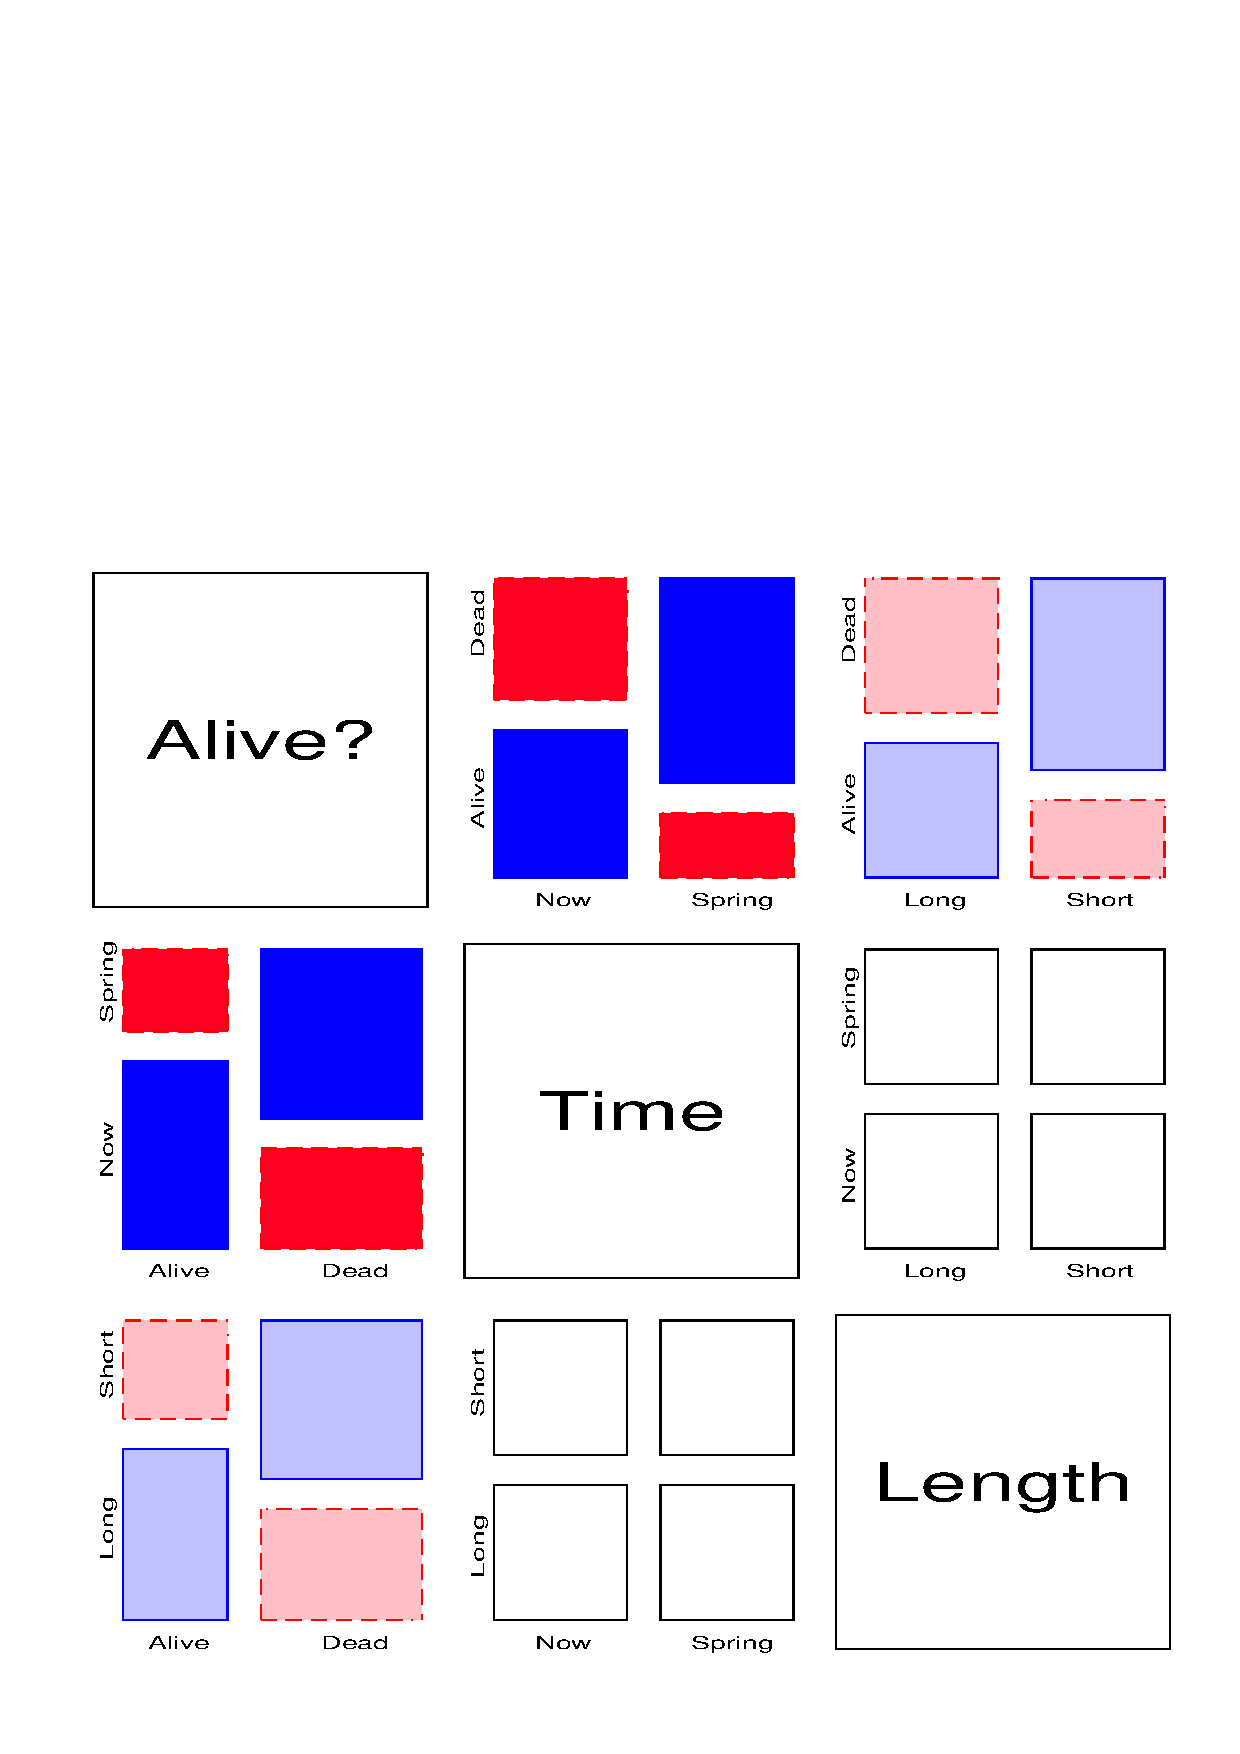
\includegraphics[scale=.7,clip]{ch5/fig/mosmat1m}
  \caption{Mosaic matrix for marginal associations in Bartlett's data}\label{fig:mosmat1m}
\end{figure}
The standard MCA analysis is carried out with the statements below.
In the call to the \macro{CORRESP}, the \mparm{INTERP=VEC}{CORRESP}
draws vectors from the origin to each main category point.
The macro produces the graph of the 2D solution shown in \figref{fig:mcabart1}; the principal inertias are shown in
\outref{out:mcabart1}.
%% input: /Users/friendly/sasuser/catdata/mcabart.sas
%% last modified: 26-Jul-99 10:48
\begin{listing}
data bartlett;
   do alive='Alive', 'Dead';
      do time='Now   ', 'Spring';
         do Length = 'Long ', 'Short';
            input count @;
            output;
            end;
         end;
      end;
datalines;
 156 107  84  31
  84 133 156 209
;
*-- Ordinary MCA of the three variables;
%corresp(data=bartlett, tables=Alive Time Length, weight=count,
   options=mca short, interp=vec, inc=0.2, pos=-,
   symbols=dot, colors=black, m0=0);
\end{listing}


\begin{figure}[htb]
  \centering
  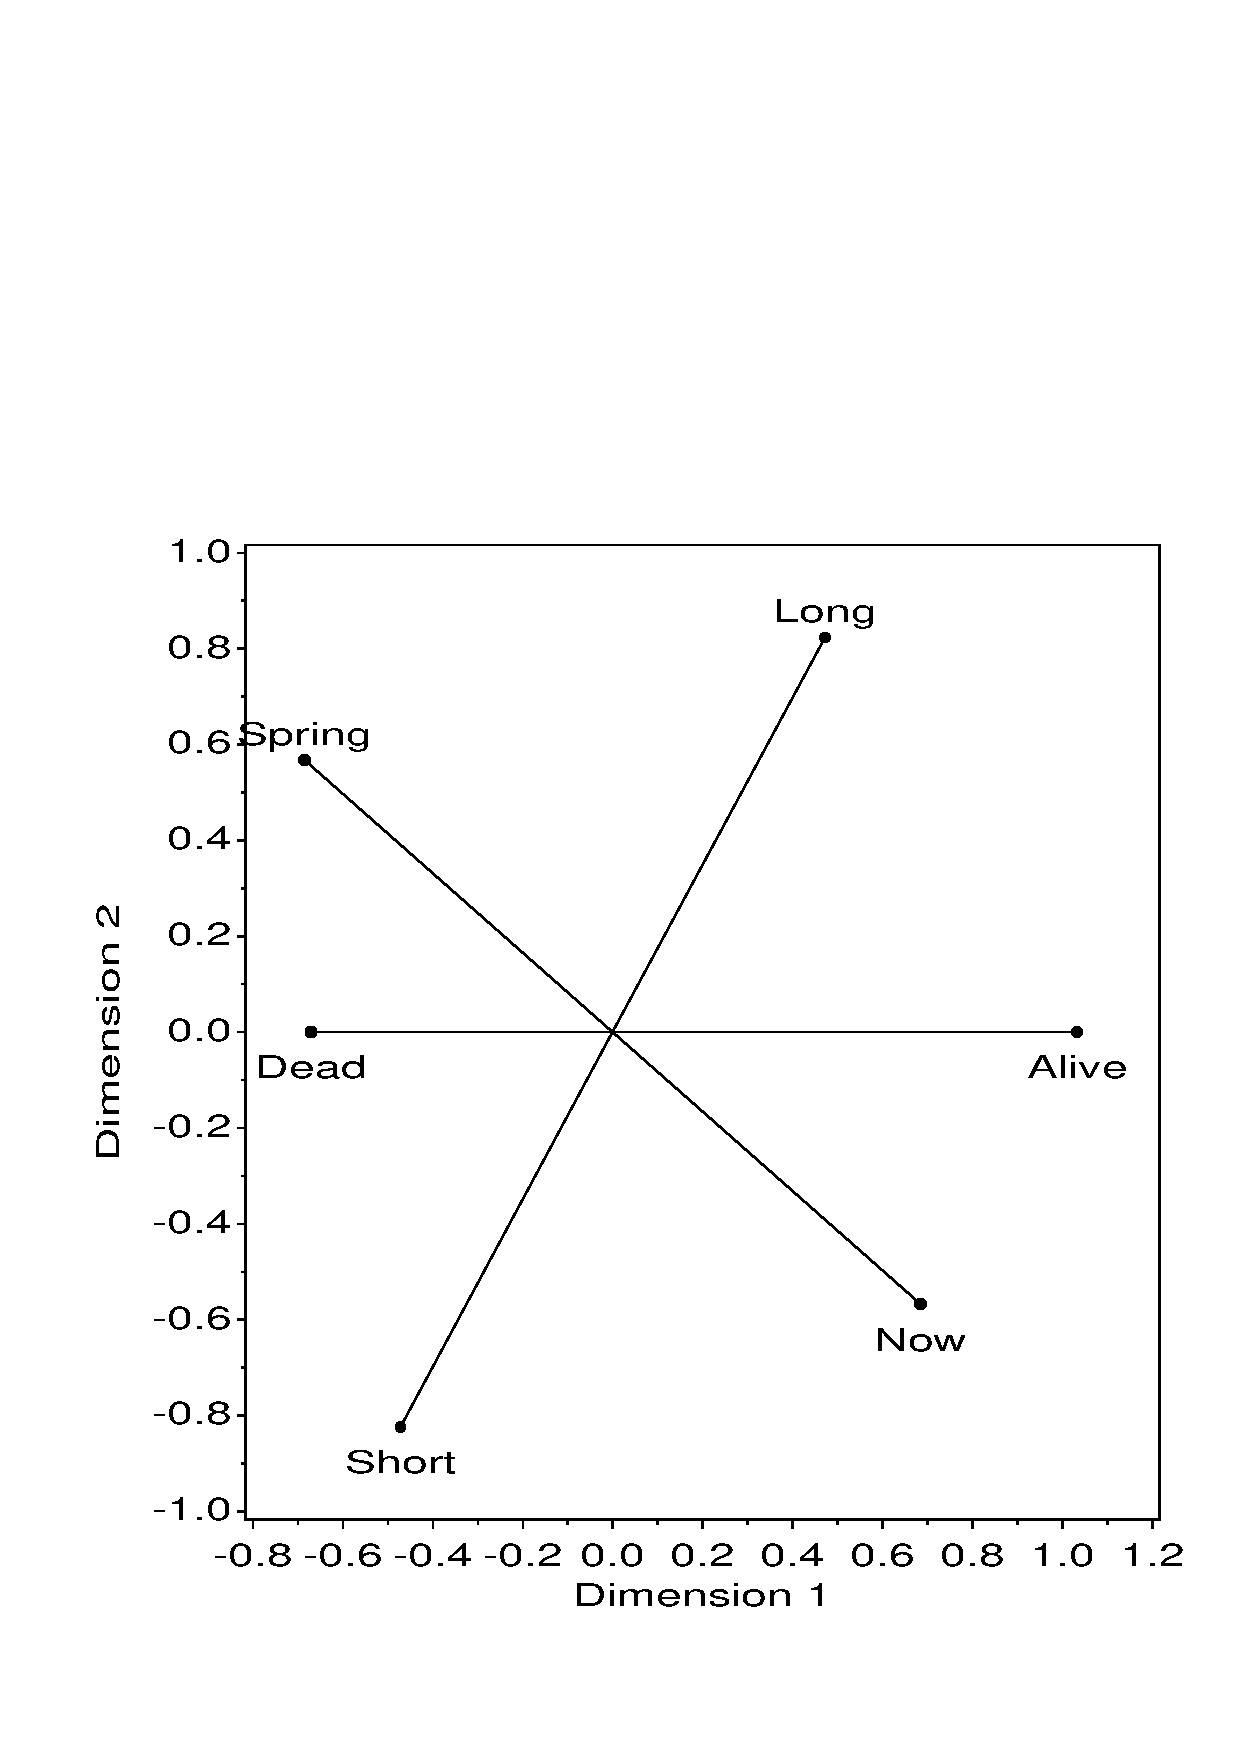
\includegraphics[scale=.7,clip]{ch5/fig/mcabart1}
  \caption{2D MCA solution for Bartlett's data}\label{fig:mcabart1}
\end{figure}

The interpretation of \figref{fig:mcabart1} is quite simple.
Dimension 1 is perfectly aligned with the Alive response variable.
The associations [AT] and [AL] of Time and Length are shown by their projections
(coordinates) on this axis.
Time has a stronger association, so its projection on this axis is larger,
and planting Long cuttings, Now leads to increased survival.
The independence of Time and Length is shown by the nearly
right angle between their vectors.%
\footnote{In an equated 3D representation, they \emph{are} orthogonal.}
Because the second principal inertia in \outref{out:mcabart1}
equals $1/Q = 1/3$ we do not interpret the second dimension.
\begin{Output}[htb]
\caption{Chi-Square Decomposition for Bartlett's data, MCA}\label{out:mcabart1}
\begin{output}
                      Inertia and Chi-Square Decomposition

        Singular  Principal Chi-
        Values    Inertias  Squares Percents    9   18   27   36   45
                                            ----+----+----+----+----+---
        0.67902   0.46107   1457.90  46.11% **************************
        0.57735   0.33333   1053.99  33.33% *******************
        0.45342   0.20559    650.08  20.56% ***********
                  -------   -------
                  1.00000   3161.97 (Degrees of Freedom = 25)
\end{output}
\end{Output}
Note also how the odds are shown by distance ratios in the plot.
Both Time and Length have equal marginal frequencies for their two
levels (odds = 1), and the ratio of distances to the origin for
the levels of both variables equals 1.0.
The ratio of distances to the origin for Alive and Dead
is inversely related to their marginal frequencies.

The statements below illustrate one way to construct the interaction
variables representing the first-order associations [AT], [AL], and [TL]
and the second-order interaction, [ATL].
Each of the character variables \pname{ALIVE}, \pname{TIME},
and \pname{LENGTH} is used to create a dummy (0/1) variable
(\pname{A}, \pname{T}, and \pname{L}, respectively).
The interaction terms are then created with binary arithmetic
in the \Dstp\ \pname{COMBO}.
A \PROC{FORMAT} step is used to create short character labels for the
combinations, to be used in the plots which follow.
These labels use an upper case letter to refer to the first level of
each main variable and a lower case letter to refer to the second level.

The \Dset\ \pname{COMBO} which results is shown in \outref{out:mcabart2}.
Note that the variables \pname{A--ATL} are actually numeric, but are printed
using their formatted values.%
\footnote{Because the interaction
variables need only be discrete, they could be created more easily, simply
by concatenating the main variables,
(e.g., \texttt{AT = ALIVE || TIME;}, and so forth).  This would produce
cluttered displays, however, because each combination is plotted and labeled.}
%
%% input: /users/faculty/friendly/sasuser/catdata/mcabart.sas
%% last modified: 13-Aug-98 17:34
\begin{listing}
*-- Formats for higher-order effects;
proc format;
   value a  0='a' 1='A';
   value t  0='t' 1='T';
   value l  0='l' 1='L';
   
   value at 0='at' 1='aT' 2='At' 3='AT';
   value al 0='al' 1='aL' 2='Al' 3='AL';
   value tl 0='tl' 1='tL' 2='Tl' 3='TL';
   value atl 0='atl' 1='atL' 2='aTl' 3='aTL' 4='Atl' 5='AtL' 6='ATl' 7='ATL';

*-- Code combinations of variables;
data combo;
   set bartlett;
   
   a = (alive='Alive');
   t = (time='Now');
   l = (length='Long');
   
   at = 2*a + t;
   al = 2*a + l;
   tl = 2*t + l;
   
   atl = 4*a + 2*t + l;
   format a a. t t. l l.  at at.  al al.  tl tl.  atl atl.;
proc print noobs;

\end{listing}

\begin{Output}[htb]
\caption{\Dset\ \pname{COMBO}: Interactive coding for Bartlett's data, Extended MCA}\label{out:mcabart2}
\begin{output}
   LENGTH    TIME      ALIVE    COUNT    A    T    L    AT    AL    TL    ATL

   Long      Now       Alive     156     A    T    L    AT    AL    TL    ATL
   Long      Now       Dead       84     a    T    L    aT    aL    TL    aTL
   Long      Spring    Alive      84     A    t    L    At    AL    tL    AtL
   Long      Spring    Dead      156     a    t    L    at    aL    tL    atL
   Short     Now       Alive     107     A    T    l    AT    Al    Tl    ATl
   Short     Now       Dead      133     a    T    l    aT    al    Tl    aTl
   Short     Spring    Alive      31     A    t    l    At    Al    tl    Atl
   Short     Spring    Dead      209     a    t    l    at    al    tl    atl
\end{output}
\end{Output}

Applying MCA to this \Dset\ using the main effect variables \pname{A T L}
would produce results identical to \figref{fig:mcabart1}.
Adding the three two-way variables, \pname{AT AL TL} will add $3 \times 4$
category points for the pairwise combinations of these factors.
The three-way variable, \pname{ATL}, adds an additional
8 category points, representing the individual cells in the table.

The analysis shown below excludes the three-way \pname{ATL} terms for simplicity.
As long as the terms are added in a balanced way
(including all terms of a given order), the positions of points tend to be very
similar whether or not terms of higher-order are included.

%% input: /users/faculty/friendly/sasuser/catdata/mcabart.sas
%% last modified: 16-Aug-98 12:26
\begin{listing}
proc corresp data=combo  mca outc=coords short;
   weight count;
   tables a t l at al tl;* atl;

*-- Identify the size and name of each effect;
data coords;
   set coords;
   where (_type_) = 'VAR';
   drop _type_ inertia contr1--best;
   terms=length(_name_);
   effect = upcase(_name_);
   label dim1 = 'Dimension 1'
         dim2 = 'Dimension 2';
proc sort;
   by terms effect _name_;
proc print;
   id _name_ effect terms;
   var dim1 dim2 mass;
\end{listing}

The \ODS\ \pname{COORDS} is used to produce the plots
shown in \figref{fig:mcabart2}.
In order to draw the vectors for the main effect points,
and quadrilaterals for the two-way terms
as in \figref{fig:mcaidemo}, variables \pname{TERMS} and \pname{EFFECT}
are added to the \pname{COORDS} \Dset\ as shown above.

%% two subfig side-by-side
\begin{figure}[htb]
 \begin{minipage}[t]{.49\linewidth}
  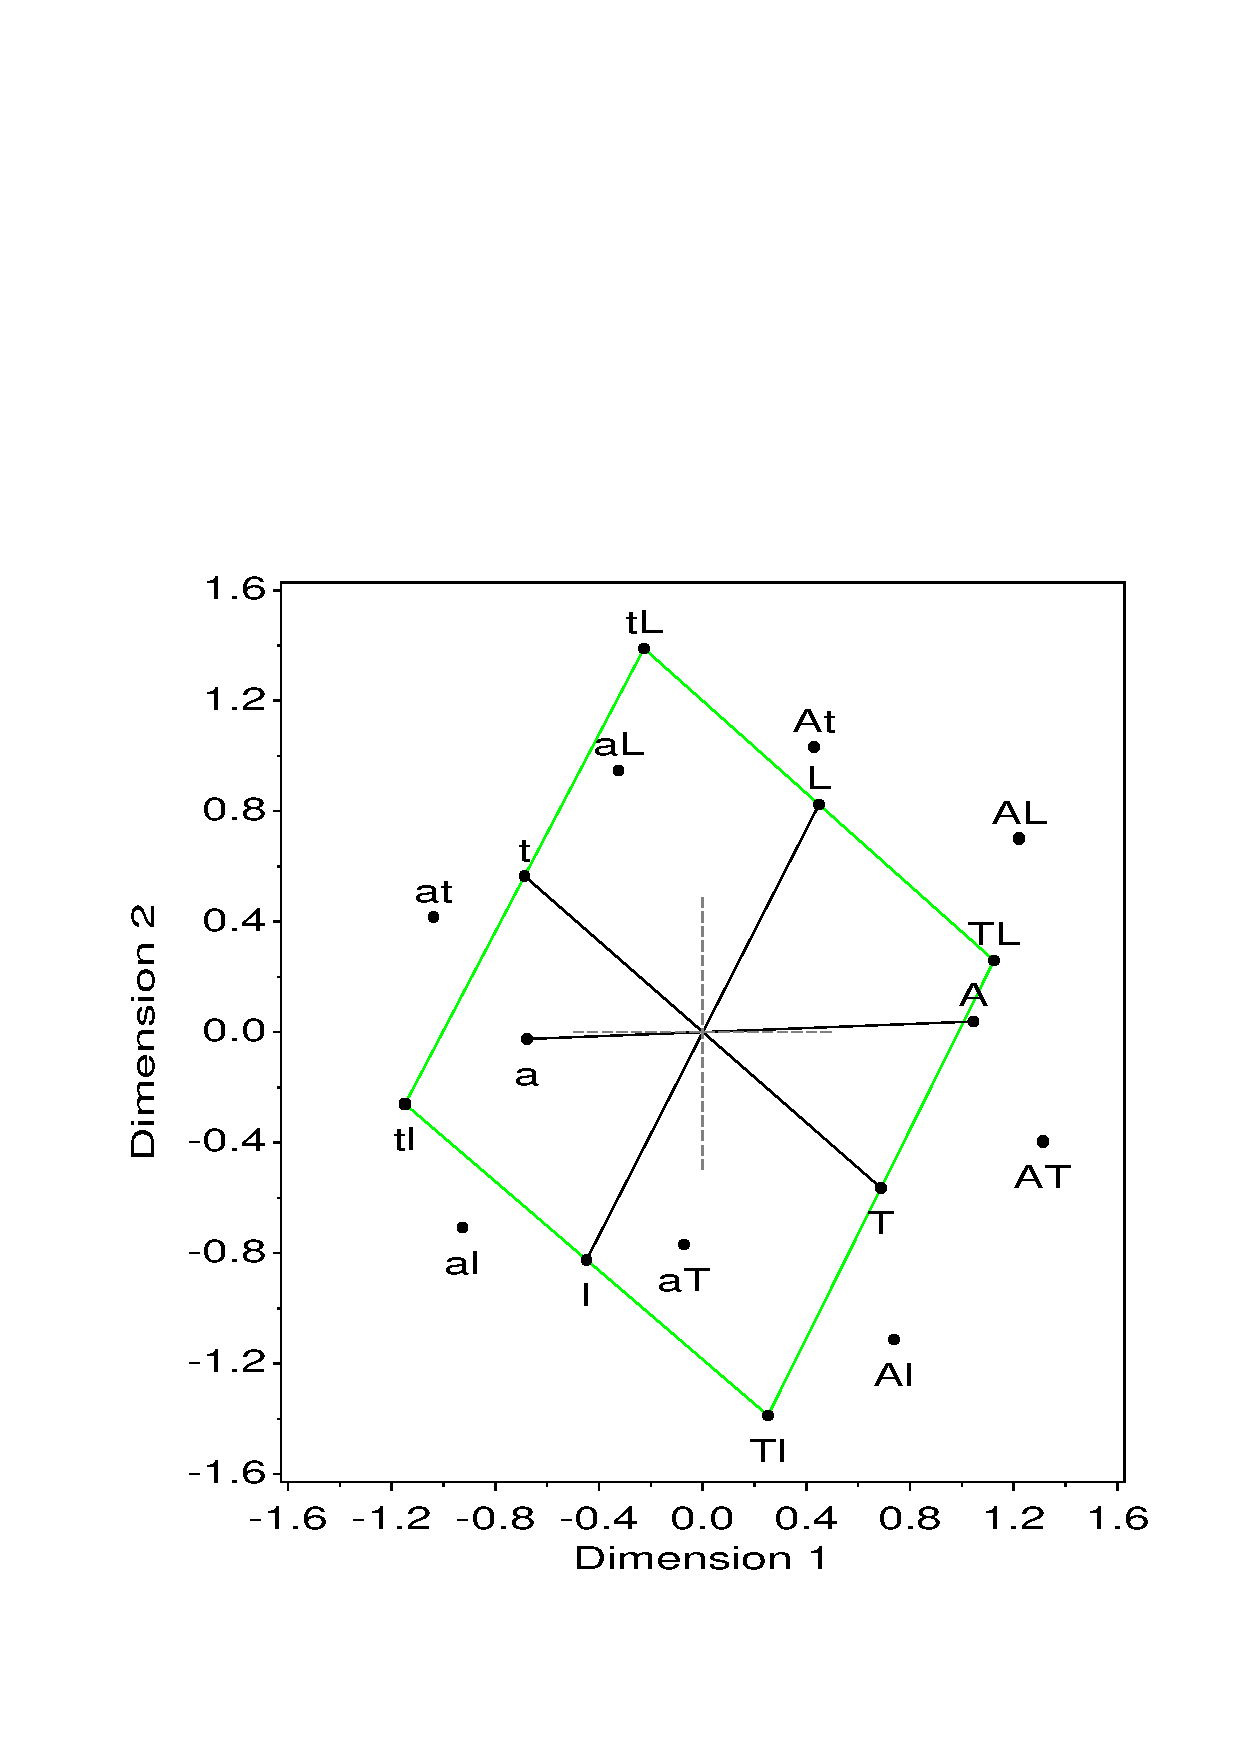
\includegraphics[width=1\linewidth]{ch5/fig/mcabart2}
 \end{minipage}%
 \hfill
 \begin{minipage}[t]{.49\linewidth}
  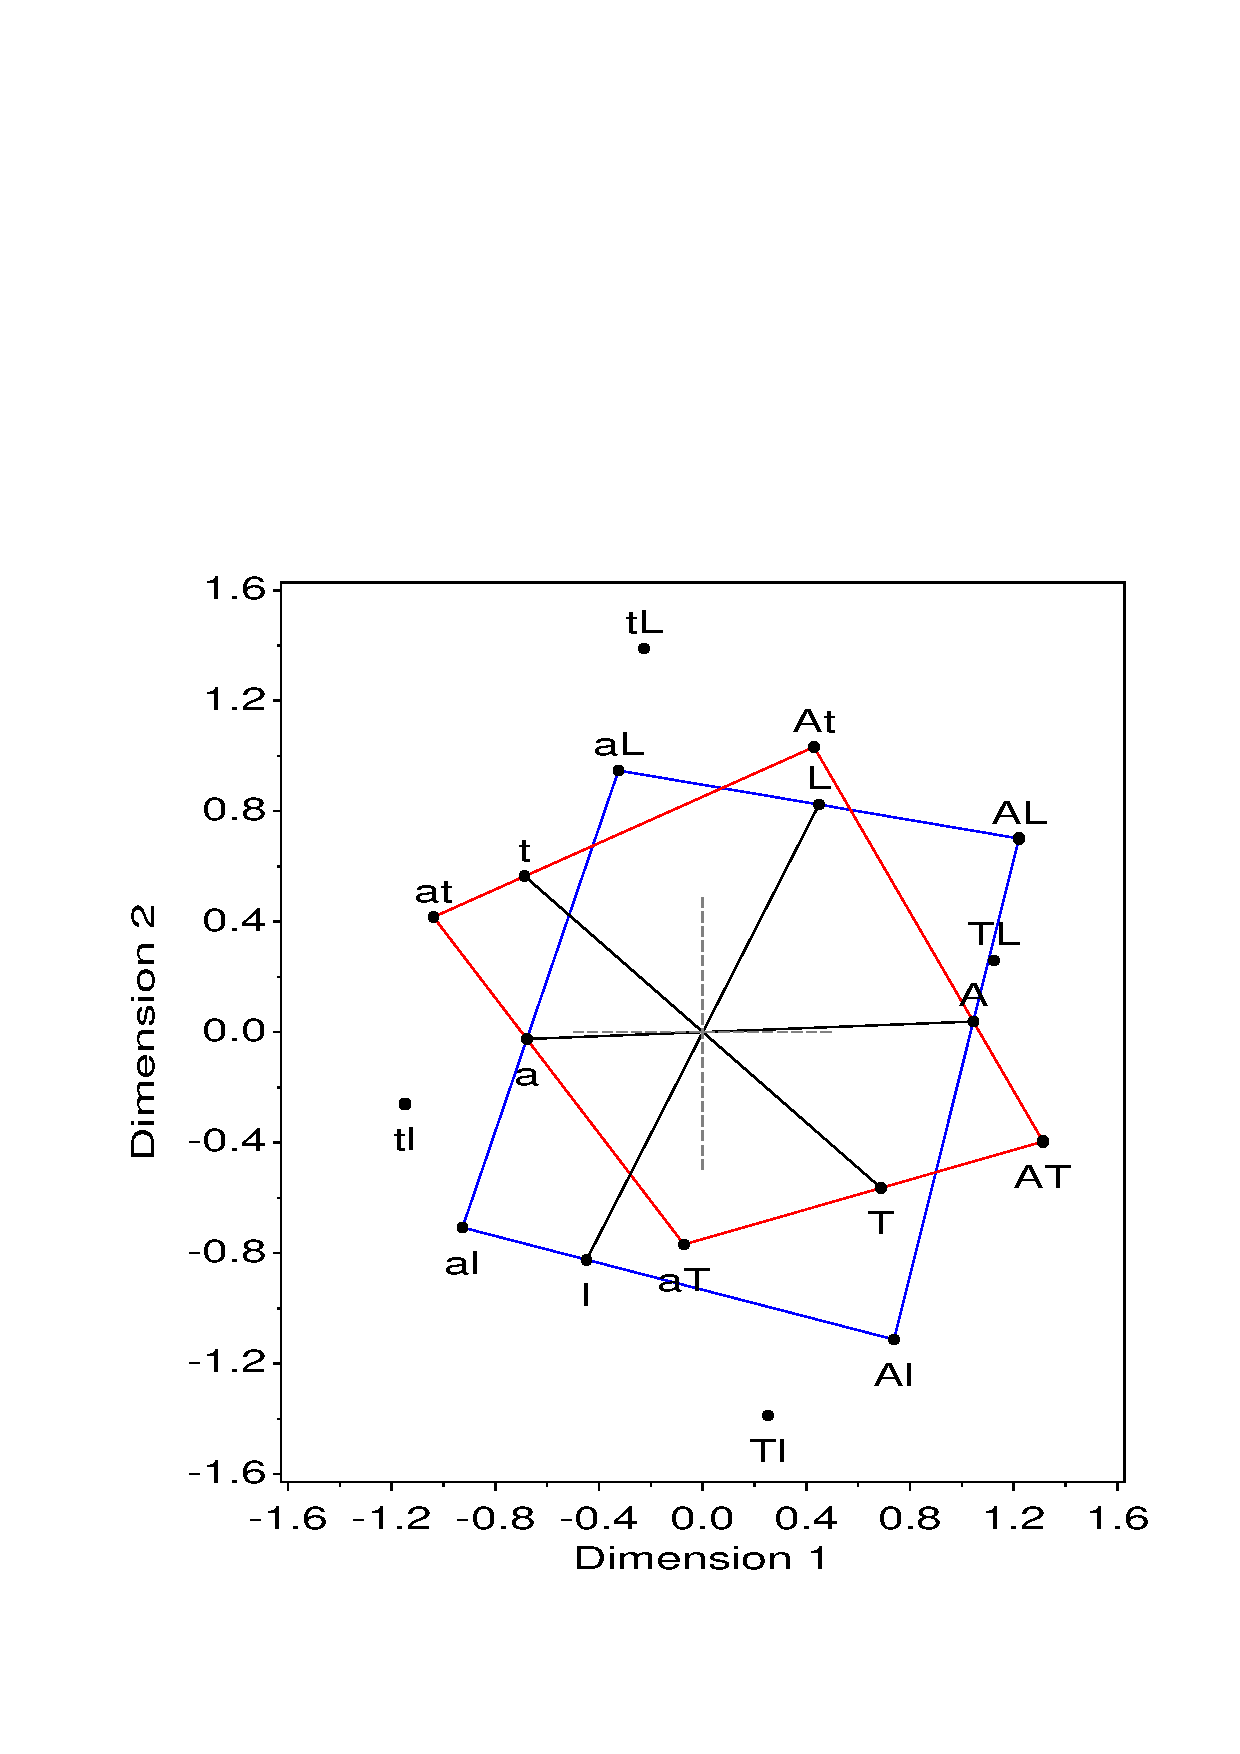
\includegraphics[width=1\linewidth]{ch5/fig/mcabart3}
 \end{minipage}
 \caption[2D Interaction display for Bartlett's data]{2D Interaction display for Bartlett's data.  Both panels show the same 2D solution for the MCA analysis including pairwise interaction effects.  In the left panel, points corresponding to the TL association are connected; lines joining the one-way
points are parallel to the sides, showing independence.
In the right panel, points for both the AT and AL associations are connected.}\label{fig:mcabart2}
\end{figure}
The following steps construct an \ADS\ to draw a quadrilateral for
each of the AT, AL and TL effects.
To do this, it is necessary to extract the \pname{DIM1} and \pname{DIM2}
of the four points for each effect and transpose these to a single
observation with variables \pname{X1-X4} and \pname{Y1-Y4} respectively.
The \Dset\ \pname{QUADS} created here is shown in \outref{out:mcabart4}
%% input: /users/faculty/friendly/sasuser/catdata/mcabart.sas
%% last modified: 16-Aug-98 12:31
\begin{listing}
*-- Extract x,y coordinates of two-way effects;
proc transpose data=coords(drop=_name_) out=quadx prefix=x;
   where (terms=2);
   var dim1;
   by effect;
proc transpose data=coords(drop=_name_) out=quady prefix=y;
   where (terms=2);
   var dim2;
   by effect;
data quads;
   merge quadx quady;
   drop _name_ _label_;
proc print data=quads;
   format _numeric_ 5.2;
   var x1 y1 x2 y2 x3 y3 x4 y4;
   id effect;

*-- Draw quadrilaterals, connecting points in order 1, 2, 4, 3;
data quads;
   set quads;
   drop x1-x4 y1-y4 i;
   retain xsys ysys '2';
   array xx\{*\} x1 x2 x4 x3;;
   array yy\{*\} y1 y2 y4 y3;
   color = scan('blue red green', _n_);
   do i=1 to 4;
      x = xx[i];  y=yy[i];
      if i=1 then function='poly    ';
             else function='polycont';
      output;
      end;

\end{listing}

\begin{Output}[htb]
\caption{\Dset\ \pname{QUADS}, containing the coordinates of the quadrilateral for each two-way effect}\label{out:mcabart4}
\begin{output}
   EFFECT     X1     Y1     X2     Y2     X3     Y3     X4     Y4

     AL     1.22   0.70   0.74  -1.11  -0.32   0.95  -0.93  -0.71
     AT     1.31  -0.40   0.43   1.03  -0.07  -0.77  -1.04   0.42
     TL     1.12   0.26   0.25  -1.39  -0.23   1.39  -1.15  -0.26
\end{output}
\end{Output}
The steps below complete the custom programming to display the TL
effect, with point labels and vectors for the main effects, in the left panel of \figref{fig:mcabart2}.
%% input: /users/faculty/friendly/sasuser/catdata/mcabart.sas
%% last modified: 16-Aug-98 12:31
\begin{listing}
%label(data=coords, out=label, x=dim1, y=dim2, text=_name_, pos=-);

data lines;
   set coords end=eof;;
   by terms effect notsorted;
   drop dim1 dim2 quality mass;
   x = dim1;
   y = dim2;
   xsys = '2'; ysys='2';

   if terms = 1  then do;
   color = 'black';
   if mod(_n_,2) = 1
      then do; function='MOVE    '; output; end;
      else do; function='DRAW    '; output; end;
   end;   

   if eof then do;
      color='gray'; line=3;
      x=-.5;  y=0;   function='MOVE';  output;   
      x=+.5;  y=0;   function='DRAW';  output;   
      x= 0 ;  y=-.5; function='MOVE';  output;   
      x= 0 ;  y=+.5; function='DRAW';  output;
      end;   
run;

*-- Show the Time X Length effect;
data anotes;
   set label lines quads(where=(effect in ('TL')));

proc gplot data=coords;
   plot dim2 * dim1 
      / frame vaxis=axis1 haxis=axis2 hm=1 vm=1
      anno=anotes;
   symbol1 v=dot h=1;
   axis1  length=6in order=(-1.6 to 1.6 by .4) label=(a=90);
   axis2  length=6in order=(-1.6 to 1.6 by .4);
run;
\end{listing}

The right panel of \figref{fig:mcabart2} is produced
using the same \PROC{GPLOT} step,
but the \ADS\ \pname{ANOTES} is assembled using just the
lines to connect the AT and AL points:
\begin{listing}
*-- Show effects on Alive;
data anotes;
   set label lines quads(where=(effect in ('AL' 'AT')));
proc gplot data=coords;
   ...
\end{listing}

Thus, we see that independence of Time and Length (by design of the
data collection) is characterized by a parallelogram shape for the
two-way points, and by lines joining the A and T one-way points
being parallel to those connecting the two-way points.
Note also that the one-way points are in essentially the same positions
as in \figref{fig:mcabart1}.
The quadrilaterals for the AT and AL effects shown in the right panel
are not quite parallelograms, however;  we could approximate the odds
ratio for each of these effects from the cross-product of distances
as in \eqref{eq:mcainter4}.
Finally, because one of the three quadrilaterals shows parallelism,
we conclude from \figref{fig:mcabart2} that the conditional independence
model, [AT][AL], holds.

An alternative representation allows us to show the cells instead, corresponding
to the ATL terms which were not displayed in \figref{fig:mcabart2}.
\begin{figure}[htb]
  \centering
  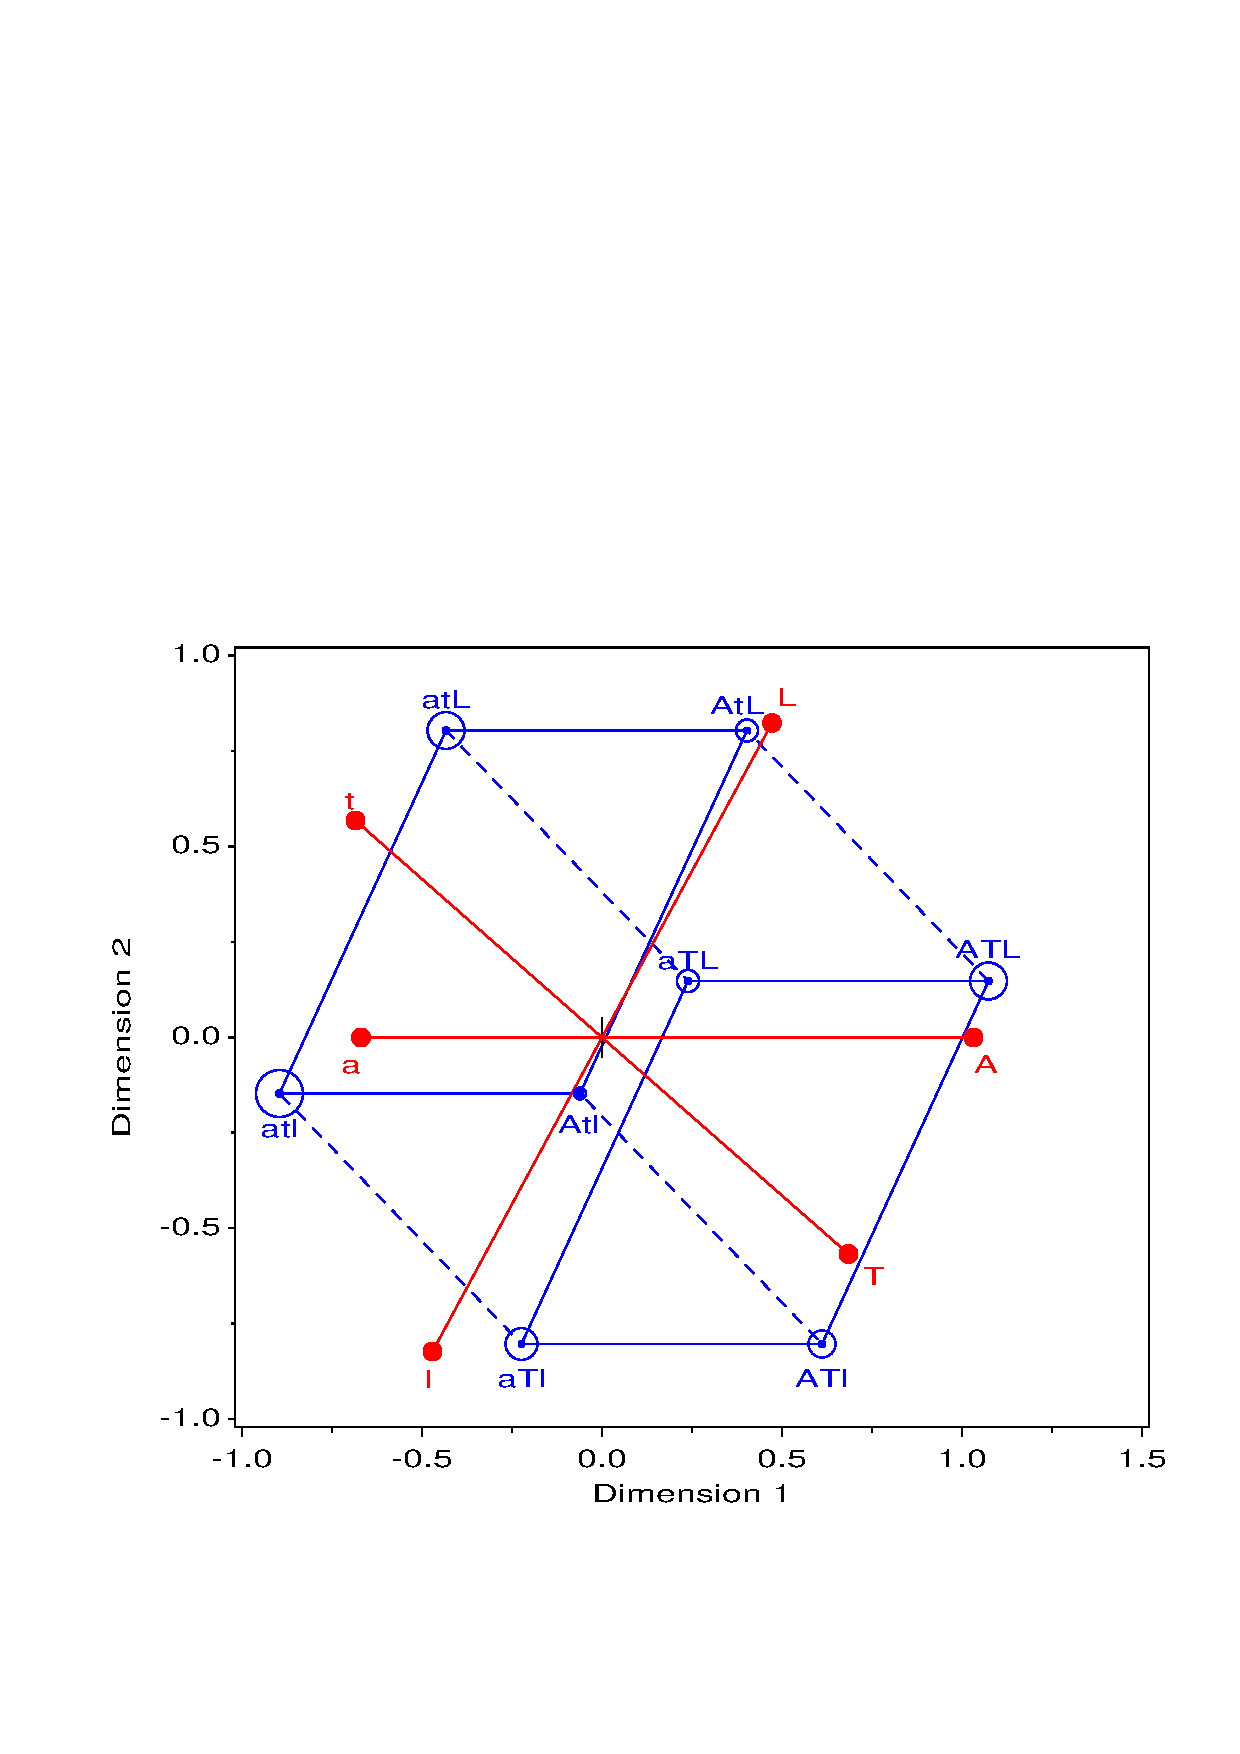
\includegraphics[scale=.7,clip]{ch5/fig/mcagen1}
  \caption[2D representation of the cell points in the $2\times 2 \times 2$ design]{2D representation of the cell points in the $2\times 2 \times 2$ design.  The mass (cell proportion) of each point is shown by the size of the circle.}\label{fig:mcagen1}
\end{figure}
We form the indicator matrix for the main effects,
$\mat{Z} = [
 \mat{Z}_A  \mat{Z}_T  \mat{Z}_L ]$,
and multiply by a diagonal matrix of the cell frequencies, to give:
\begin{output}
   ID    ALIVE   TIME     LENGTH   COUNT    A1    A2    T1    T2    L1    L2

   ATL   Alive   Now      Long      156    156     0   156     0   156     0
   aTL   Dead    Now      Long       84      0    84    84     0    84     0
   AtL   Alive   Spring   Long       84     84     0     0    84    84     0
   atL   Dead    Spring   Long      156      0   156     0   156   156     0
   ATl   Alive   Now      Short     107    107     0   107     0     0   107
   aTl   Dead    Now      Short     133      0   133   133     0     0   133
   Atl   Alive   Spring   Short      31     31     0     0    31     0    31
   atl   Dead    Spring   Short     209      0   209     0   209     0   209
\end{output}
Then, a simple \CA\ of the variables \pname{A1--L2} will have row points
corresponding to the cells, and column for the main effects which are
nearly identical to those from the extended MCA.
This analysis produces the display in \figref{fig:mcagen1}
(program steps are not shown to conserve space), where the
size of the circle at each point represents the mass ($p_{ijk}$) of each
cell, whose label is the \pname{ID} variable above.
The two-way points can be added to this representation by including the two-way indicator matrices, so we analyze the matrix
$\diag (\vec{n}) [
 \mat{Z}_A  \mat{Z}_T  \mat{Z}_L  \mat{Z}_{AT}
 \mat{Z}_{AL}  \mat{Z}_{TL}
]$.
\end{Example}
\ixoff{multiple correspondence analysis!extended}
